\uuid{oaC1}
\exo7id{5533}
\auteur{rouget}
\organisation{exo7}
\datecreate{2010-07-15}
\isIndication{false}
\isCorrection{true}
\chapitre{Courbes planes}
\sousChapitre{Coordonnées polaires}

\contenu{
\texte{
Construire la courbe d'équation cartésienne $x^2(x^2+y^2)-(y-x)^2=0$ après être passé en polaires .
}
\reponse{
Soient $(R,\theta)\in\Rr^2$ puis $M$ le point du plan dont un couple de coordonnées polaires est $[r,\theta]$.

\begin{align*}\ensuremath
M\in\mathcal{C}&\Leftrightarrow x^2(x^2+y^2)-(y-x)^2=0
\Leftrightarrow r^2\cos^2\theta\times r^2-(r\sin\theta-r\cos\theta)^2=0\\
 &\Leftrightarrow r^2[r^2\cos^2\theta-(\sin\theta-\cos\theta)^2]=0\Leftrightarrow r=0\;\text{ou}\;r^2=\left(\frac{\sin\theta-\cos\theta}{\cos\theta}\right)^2\;(\cos\theta=0\;\text{ne fournit pas de solution})\\
 &\Leftrightarrow r=0\;\text{ou}\;r=\tan\theta-1\;\text{ou}\;r=1-\tan\theta.
\end{align*}
$\mathcal{C}$ est donc la réunion de la courbe $(\mathcal{C}_1)$ d'équation polaire $r=\tan\theta-1$, $(\mathcal{C}_2)$ d'équation polaire $r=1-\tan\theta$ et $\{O\}$.
On note que le point $O$ appartient à $(\mathcal{C}_1)$ car $\theta=\frac{\pi}{4}$ fournit $r=0$. Donc $\mathcal{C}=\mathcal{C}_1\cup\mathcal{C}_2\cup\{O\}=\mathcal{C}_1\cup\mathcal{C}_2$. Ensuite, on notant $r_1$ et $r_2$ respectivement la fonction $\theta\mapsto\tan\theta-1$ et $r_2=-r_1$,

\begin{center}
$M[\theta+\pi,r_2(\theta+\pi)]=M[\theta+\pi,r_2(\theta)]=M[\theta+\pi,-r_1(\theta)]=M[\theta,r_1(\theta)]$,
\end{center}
et comme $\theta+\pi$ décrit $\Rr$ si et seulement si $\theta$ décrit $\Rr$, les courbes $\mathcal{C}_1$ et $\mathcal{C}_2$ sont une seule et même courbe.

\begin{center}
\shadowbox{
$\mathcal{C}$ est la courbe d'équation polaire $r=\tan\theta-1$.
}
\end{center}
\textbf{Construction de $\mathcal{C}$.}

$$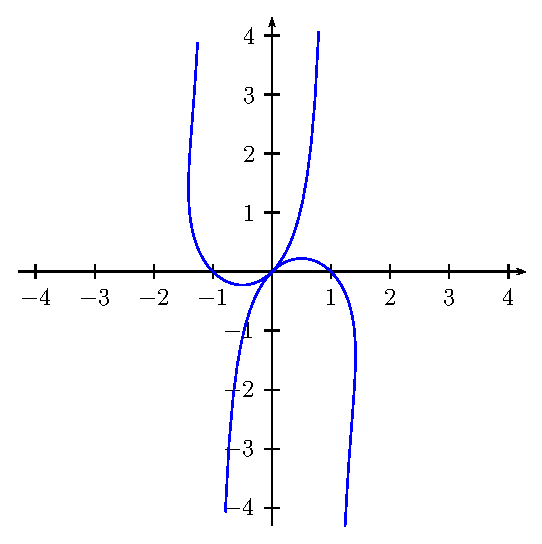
\includegraphics{../images/img005533-1}$$
}
}
